Sigui la funció $f(x)=\dfrac1x$.

\begin{apartats}

\apartat{0,75}
Calculeu l'equació de la recta tangent a la gràfica de la funció $f$ en el punt d'abscissa $x=2$.

\begin{solucio}
$f(x)=\frac1x$ i $f'(x)=-\frac{1}{x^2}$. La recta passa pel punt $(2,f(2))=\left(2,\frac12\right)$, i el seu
pendent és $f'(2)=-\frac14$:
\[
y-\frac12=-\frac14\,(x-2)\;\Rightarrow\;y=-\frac x4+\frac24+\frac12 .
\]
Per tant, la recta tangent és $\boxed{y=-\frac x4+1}$.

\textit{Pauta oficial:} 0,25 per trobar el punt, 0,25 per trobar el pendent i 0,25 per trobar la recta tangent.
\end{solucio}

\apartat{0,75}
Calculeu l'equació de la recta tangent a la gràfica de la funció $f$ en el punt d'abscissa $x=k$, en què $k$ és un
nombre real positiu.

\begin{solucio}
La recta passa pel punt $(k,f(k))=\left(k,\frac1k\right)$, i el seu pendent és $f'(k)=-\frac{1}{k^2}$:
\[
y-\frac1k=-\frac{1}{k^2}\,(x-k)\;\Rightarrow\;y=-\frac{x}{k^2}+\frac2k .
\]
Per tant, la recta tangent és $\boxed{y=-\frac{x}{k^2}+\frac2k}$.

\textit{Pauta oficial:} 0,25 per trobar el punt, 0,25 per trobar el pendent i 0,25 per trobar la recta tangent
(en funció de $k$).
\end{solucio}

\apartat{1}
Comproveu que, tal com es pot veure en la figura de sota, la recta de l'apartat b) determina un triangle d'àrea
constant amb els semieixos positius de coordenades. Calculeu aquesta àrea.
\begin{center}
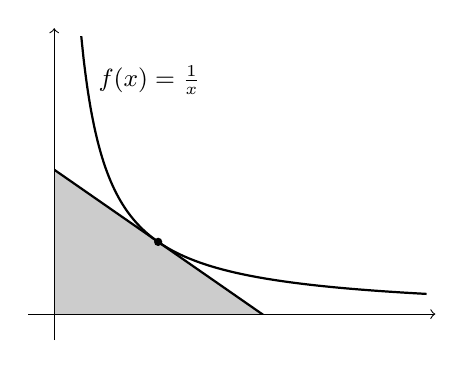
\begin{tikzpicture}[x=1.1cm,y=1.1cm]
  \fill[gray!40] (0,0) -- (2.4,0) -- (0,1.6667) -- cycle;
  \draw[->] (-0.3,0) -- (4.4,0);
  \draw[->] (0,-0.3) -- (0,3.3);
  \begin{scope}
    \clip (0,0) rectangle (4.4,3.2);
    \draw[\colorgrafica,thick,domain=0.3:4.3,samples=100,smooth] plot (\x,{1/\x});
    \draw[thick] (-0.1,1.7361) -- (2.7,-0.2083);
  \end{scope}
  \fill (1.2,0.8333) circle (1.5pt);
  \node[font=\small] at (1.1,2.7) {$f(x)=\frac1x$};
\end{tikzpicture}
\end{center}

\begin{solucio}
Calculem els punts de tall de la recta tangent, $y=\frac2k-\frac{x}{k^2}$, amb l'eix d'abscisses i amb l'eix
d'ordenades:
\[
\left\{\begin{aligned}y&=\tfrac2k-\tfrac{x}{k^2}\\y&=0\end{aligned}\right.\;\rightarrow\;(2k,0),\qquad
\left\{\begin{aligned}y&=\tfrac2k-\tfrac{x}{k^2}\\x&=0\end{aligned}\right.\;\rightarrow\;\left(0,\tfrac2k\right).
\]
Per tant,
\[
\text{Àrea del triangle}=\frac12\cdot2k\cdot\frac2k=2\ \text{u}^2 .
\]
El triangle té àrea constant, igual a 2 unitats de superfície, per a qualsevol valor del paràmetre $k$.

\textit{Pauta oficial:} 0,25 per trobar el punt de tall amb l'eix de les abscisses, 0,25 per trobar el punt de
tall amb l'eix de les ordenades, 0,25 per trobar el valor de l'àrea i 0,25 per expressar que l'àrea és constant
per a qualsevol valor del paràmetre $k$.
\end{solucio}

\end{apartats}
